\documentclass[border=12pt]{standalone}
\usepackage{tikz}
\usepackage{amsmath}
\usetikzlibrary{arrows.meta, positioning, calc, fit, backgrounds, shapes.geometric}

\definecolor{initblue}{HTML}{2E86C1}
\definecolor{compgreen}{HTML}{239B56}
\definecolor{propurple}{HTML}{7D3C98}
\definecolor{outred}{HTML}{C0392B}
\definecolor{dataorange}{HTML}{D68910}
\definecolor{bglight}{HTML}{F7F9F9}

\tikzset{
    startstop/.style={
        rectangle, rounded corners=8pt, minimum width=4.7cm, minimum height=0.95cm,
        align=center, draw=black, line width=1pt, fill=initblue!14, font=\bfseries\small
    },
    process/.style={
        rectangle, rounded corners=4pt, minimum width=4.9cm, minimum height=0.95cm,
        align=center, draw=black, line width=0.8pt, fill=compgreen!10,
        font=\small, text width=4.6cm
    },
    propagate/.style={
        rectangle, rounded corners=4pt, minimum width=4.9cm, minimum height=0.95cm,
        align=center, draw=propurple, line width=0.8pt, fill=propurple!11,
        font=\small, text width=4.6cm
    },
    output/.style={
        trapezium, trapezium left angle=72, trapezium right angle=108,
        minimum width=3.9cm, minimum height=0.95cm, align=center,
        draw=outred, line width=0.8pt, fill=outred!8, font=\small, text width=3.4cm
    },
    datafile/.style={
        cylinder, shape border rotate=90, draw=dataorange, line width=0.8pt,
        minimum height=1.0cm, minimum width=3.0cm, fill=dataorange!12,
        font=\small, aspect=0.25, align=center
    },
    arrow/.style={-Stealth, thick, draw=black!70},
    dasharrow/.style={-Stealth, thick, dashed, draw=black!55},
    groupbox/.style={
        draw=black!30, dashed, rounded corners=6pt, inner sep=8pt,
        fill=bglight, fill opacity=0.55
    },
    grouplabel/.style={font=\bfseries\footnotesize, text=black!65}
}

\begin{document}
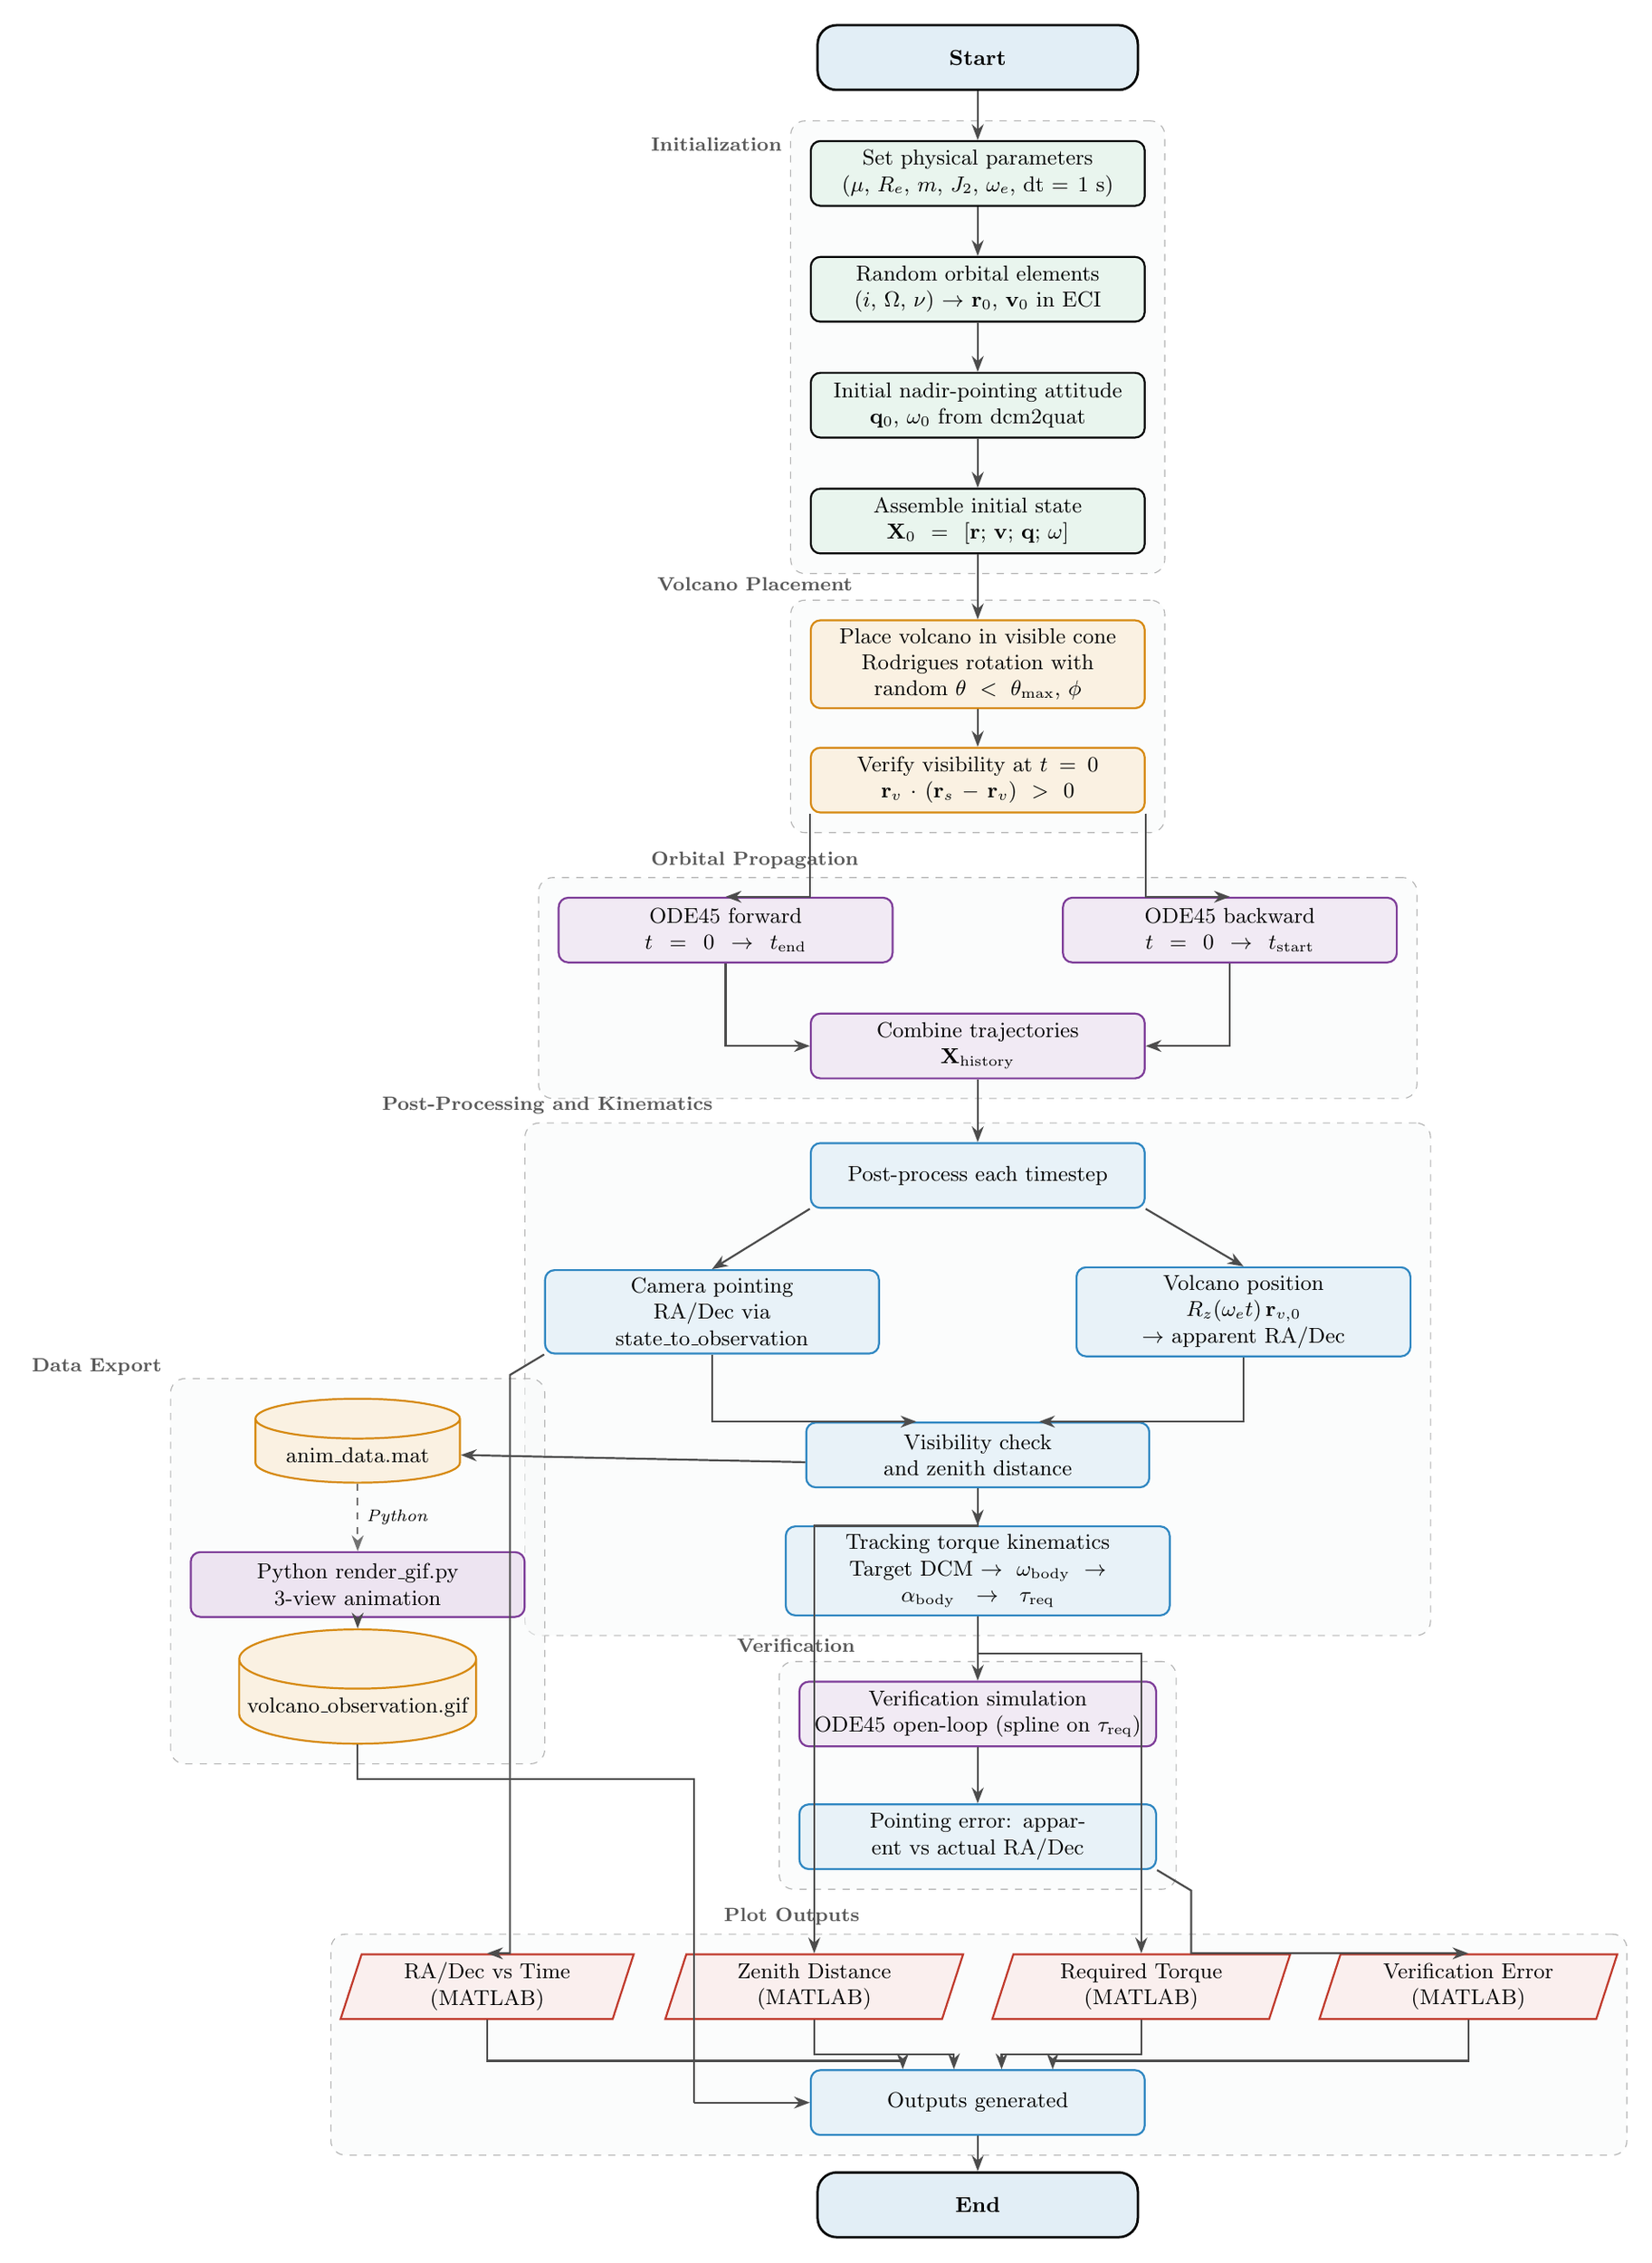
\begin{tikzpicture}[x=1cm, y=1cm]

% === INITIALIZATION ===
\node (start)   [startstop] at (0, 0.0)   {Start};
\node (params)  [process]   at (0,-1.7)   {Set physical parameters\\($\mu$, $R_e$, $m$, $J_2$, $\omega_e$, dt $=1$ s)};
\node (orbit)   [process]   at (0,-3.4)   {Random orbital elements\\($i$, $\Omega$, $\nu$) $\to$ $\mathbf{r}_0$, $\mathbf{v}_0$ in ECI};
\node (att)     [process]   at (0,-5.1)   {Initial nadir-pointing attitude\\$\mathbf{q}_0$, $\omega_0$ from dcm2quat};
\node (state)   [process]   at (0,-6.8)   {Assemble initial state\\$\mathbf{X}_0=[\mathbf{r};\,\mathbf{v};\,\mathbf{q};\,\omega]$};

% === VOLCANO PLACEMENT ===
\node (volcano) [process, fill=dataorange!12, draw=dataorange] at (0,-8.9) {
    Place volcano in visible cone\\
    Rodrigues rotation with random $\theta<\theta_{\max}$, $\phi$
};
\node (verify0) [process, fill=dataorange!12, draw=dataorange] at (0,-10.6) {
    Verify visibility at $t=0$\\
    $\mathbf{r}_v\cdot(\mathbf{r}_s-\mathbf{r}_v)>0$
};

% === ORBITAL PROPAGATION ===
\node (propfwd) [propagate] at (-3.7,-12.8) {ODE45 forward\\$t=0 \rightarrow t_{\mathrm{end}}$};
\node (propbwd) [propagate] at ( 3.7,-12.8) {ODE45 backward\\$t=0 \rightarrow t_{\mathrm{start}}$};
\node (combine) [propagate] at (0,-14.5)    {Combine trajectories\\$\mathbf{X}_{\mathrm{history}}$};

% === POST-PROCESSING AND KINEMATICS ===
\node (post)    [process, fill=initblue!11, draw=initblue] at (0,-16.4) {Post-process each timestep};
\node (camera)  [process, fill=initblue!11, draw=initblue, text width=3.9cm] at (-3.9,-18.4) {
    Camera pointing\\RA/Dec via state\_to\_observation
};
\node (volcrot) [process, fill=initblue!11, draw=initblue, text width=3.9cm] at (3.9,-18.4) {
    Volcano position\\$R_z(\omega_e t)\,\mathbf{r}_{v,0}$\\$\to$ apparent RA/Dec
};
\node (viszen)  [process, fill=initblue!11, draw=initblue, text width=4.8cm] at (0,-20.5) {
    Visibility check and zenith distance
};
\node (torque)  [process, fill=initblue!11, draw=initblue, text width=5.4cm] at (0,-22.2) {
    Tracking torque kinematics\\
    Target DCM $\to \omega_{\mathrm{body}} \to \alpha_{\mathrm{body}} \to \tau_{\mathrm{req}}$
};

% === VERIFICATION ===
\node (verifsim) [propagate, text width=5.0cm] at (0,-24.3) {
    Verification simulation\\
    ODE45 open-loop (spline on $\tau_{\mathrm{req}}$)
};
\node (veriferr) [process, fill=initblue!11, draw=initblue, text width=5.0cm] at (0,-26.1) {
    Pointing error: apparent vs actual RA/Dec
};

% === DATA EXPORT ===
\node (savemat) [datafile] at (-9.1,-20.5) {anim\_data.mat};
\node (python)  [process, fill=propurple!14, draw=propurple, text width=4.0cm] at (-9.1,-22.4) {
    Python render\_gif.py\\3-view animation
};
\node (gif)     [datafile] at (-9.1,-24.2) {volcano\_observation.gif};

% === PLOTS ===
\node (plotRA)     [output] at (-7.2,-28.3) {RA/Dec vs Time\\(MATLAB)};
\node (plotZen)    [output] at (-2.4,-28.3) {Zenith Distance\\(MATLAB)};
\node (plotTorque) [output] at ( 2.4,-28.3) {Required Torque\\(MATLAB)};
\node (plotError)  [output] at ( 7.2,-28.3) {Verification Error\\(MATLAB)};

\node (done) [process, fill=initblue!11, draw=initblue, text width=4.0cm] at (0,-30.0) {Outputs generated};
\node (stop) [startstop] at (0,-31.5) {End};

% === MAIN FLOW ARROWS ===
\draw [arrow] (start) -- (params);
\draw [arrow] (params) -- (orbit);
\draw [arrow] (orbit) -- (att);
\draw [arrow] (att) -- (state);
\draw [arrow] (state) -- (volcano);
\draw [arrow] (volcano) -- (verify0);

\draw [arrow] (verify0.south west) |- (propfwd.north);
\draw [arrow] (verify0.south east) |- (propbwd.north);
\draw [arrow] (propfwd.south) |- (combine.west);
\draw [arrow] (propbwd.south) |- (combine.east);

\draw [arrow] (combine) -- (post);
\draw [arrow] (post.south west) -- (camera.north);
\draw [arrow] (post.south east) -- (volcrot.north);
\draw [arrow] (camera.south) |- ([xshift=-0.9cm]viszen.north);
\draw [arrow] (volcrot.south) |- ([xshift=0.9cm]viszen.north);

\draw [arrow] (viszen) -- (torque);
\draw [arrow] (torque) -- (verifsim);
\draw [arrow] (verifsim) -- (veriferr);

% === OUTPUT ARROWS ===
\draw [arrow] ([yshift=-3pt]viszen.west) -- (savemat.east);
\draw [dasharrow] (savemat.south) -- node[right, font=\scriptsize\itshape]{Python} (python.north);
\draw [arrow] (python.south) -- (gif.north);

\draw [arrow] (camera.south west) -- ++(-0.5,-0.3) |- (plotRA.north);
\draw [arrow] (viszen.south) -- ++(0,-0.55) -| (plotZen.north);
\draw [arrow] (torque.south) -- ++(0,-0.55) -| (plotTorque.north);
\draw [arrow] (veriferr.south east) -- ++(0.5,-0.3) |- (plotError.north);

\draw [arrow] (plotRA.south) -- ++(0,-0.6) -| ([xshift=-1.1cm]done.north);
\draw [arrow] (plotZen.south) -- ++(0,-0.5) -| ([xshift=-0.35cm]done.north);
\draw [arrow] (plotTorque.south) -- ++(0,-0.5) -| ([xshift=0.35cm]done.north);
\draw [arrow] (plotError.south) -- ++(0,-0.6) -| ([xshift=1.1cm]done.north);
\coordinate (gifjoin) at ([xshift=-1.7cm]done.west);
\draw [-, thick, draw=black!70] (gif.south) -- ++(0,-0.5) -| (gifjoin);
\draw [arrow] (gifjoin) -- (done.west);

\draw [arrow] (done) -- (stop);

% === GROUPS ===
\begin{scope}[on background layer]
    \node[groupbox, fit=(params)(state), label={[grouplabel]above left:Initialization}] {};
    \node[groupbox, fit=(volcano)(verify0), label={[grouplabel]above left:Volcano Placement}] {};
    \node[groupbox, fit=(propfwd)(propbwd)(combine), label={[grouplabel]above left:Orbital Propagation}] {};
    \node[groupbox, fit=(post)(camera)(volcrot)(viszen)(torque), label={[grouplabel]above left:Post-Processing and Kinematics}] {};
    \node[groupbox, fit=(verifsim)(veriferr), label={[grouplabel]above left:Verification}] {};
    \node[groupbox, fit=(savemat)(python)(gif), label={[grouplabel]above left:Data Export}] {};
    \node[groupbox, fit=(plotRA)(plotZen)(plotTorque)(plotError)(done), label={[grouplabel]above left:Plot Outputs}] {};
\end{scope}

\end{tikzpicture}
\end{document}
